%%%%%%%%%%%%%%%%%%%% SECTION %%%%%%%%%%%%%%%%%%%%%%%
\section{Rapid Review research protocol} \label{section:en/protocolo}

This section describes the research protocol used for this rapid review. Rapid Reviews (RR) are practice-oriented secondary studies, and their main goal is to provide evidence to support decision-making towards the solution, or at least attenuation, of issues practitioners face in practice \cite{Cartaxo2020}.

For this Rapid Review, the PRISMA \cite{Tricco2019} methodology was used for reference. The research question for the case study of this work, the repositories used for the search, the search process and search string, the inclusion and exclusion criteria and the selection process are specified as follows.


%%%%%%%%%%%%%%%%%%%% SECTION %%%%%%%%%%%%%%%%%%%%%%%
\subsection{Research Question}

The Research Question to be answered is the following: \emph{What are the main factors that limit the implementation of AI/xAI in histopathology?} Considering all of the impediments reported so far will permit to gather all of the known and necessary requirements to implement AI/xAI in histopathology. 




%%%%%%%%%%%%%%%%%%%% SECTION %%%%%%%%%%%%%%%%%%%%%%%
\subsection{Search Process and Search string}

An automatic search in the ACM, IEEE Xplore, PubMed and Springer digital libraries and platforms was conducted. The search included publications between January 2015 and June 2023.

For the construction of the search string, the main terms “explainable artificial intelligence”, “histopathology”, “histology” and “anatomic pathology” were considered, including their alternative terms. The resulting search string is presented in Figure \ref{figura:en/cadena_generica}.

\begin{figure}[htbp]
\centering
\begin{tabular}{c}
\begin{lstlisting}
#FULL TEXT
  "xai" OR
  "explainable artificial intelligence" OR
  "explainable ai" OR
  "interpretable ai" OR
  "interpretable artificial intelligence" OR
  "white box" OR
  "human ai"
#AND
#FULL TEXT
  "histopathology" OR
  "histopathological" OR
  "histology" OR
  "histological" OR
  "anatomic pathology" OR
  "anatomical pathology"
\end{lstlisting}
\end{tabular}
\caption{Search string defined for the research}
\label{figura:en/cadena_generica}
\end{figure}



%%%%%%%%%%%%%%%%%%%% SECTION %%%%%%%%%%%%%%%%%%%%%%%
\subsection{Inclusion and exclusion criteria}

The inclusion and exclusion criteria used for the article selection process are presented in Table \ref{tabla:en/criterios_inc_exc}.

\begin{table}[htbp]
\caption{Inclusion and exclusion criteria details}
\begin{center}
\resizebox{\columnwidth}{!}{
\begin{tabular}{| m{10em} | m{10em} |}
\hline
\textbf{Inclusion criteria} & \textbf{Exclusion criteria} \\
\hline
Articles published in English. & Articles published in languages other than English. \\ 
\hline
Articles published between January 2015 and June 2023. & Articles published before January 2015. \\
\hline
Articles published in journals or conferences that underwent peer review. & Articles that were not peer-reviewed. \\
\hline
Articles whose main focus is the implementation of AI/xAI in histology or histopathology. & Unavailable or incomplete articles. \\
\hline
& Duplicate Articles. \\
\hline
& Surveys, systematic reviews and other rapid reviews. \\
\hline
\end{tabular}}
\label{tabla:en/criterios_inc_exc}
\end{center}
\end{table}


%%%%%%%%%%%%%%%%%%%% SECTION %%%%%%%%%%%%%%%%%%%%%%%
\subsection{Selection process}

The study selection process consisted of ten steps, which were executed sequentially. Details about the process are described in Table \ref{tabla:en/proceso_busqueda}. This process allowed the selection of the primary studies that were analyzed to answer the research question.

\begin{table}[htbp]
\caption{Selection process details}
\begin{center}
\resizebox{\columnwidth}{!}{
\begin{tabular}{|m{2em}|m{20em}|}
\hline
\textbf{Step} & \textbf{Procedure} \\
\hline
{1} & {Compilation of search results, organized by repository} \\
\hline
\textbf{2} & {Selection by publication language} \\
\hline
\textbf{3} & {Selection by publication type} \\
\hline
\textbf{4} & {Elimination of duplicate results by repository} \\
\hline
\textbf{5} & {Selection by title} \\
\hline
\textbf{6} & {Collection of partial results for each repository} \\
\hline
\textbf{7} & {Elimination of duplicate results across repositories} \\
\hline
\textbf{8} & {Selection by abstract} \\
\hline
\textbf{9} & {Selection by availability of the material} \\
\hline
\textbf{10} & {Complete review} \\
\hline
\end{tabular}}
\label{tabla:en/proceso_busqueda}
\end{center}
\end{table}


%%%%%%%%%%%%%%%%%%%% SECTION %%%%%%%%%%%%%%%%%%%%%%%
\subsection{Data Extraction process}

This section presents the search performed in the digital libraries and platforms. The search string was applied in the libraries with some necessary adjustments depending on the particularities of each one. Figure \ref{figura:en/data_extraction} shows the articles search and selection process.

\begin{figure*}[t]
    \centering
%    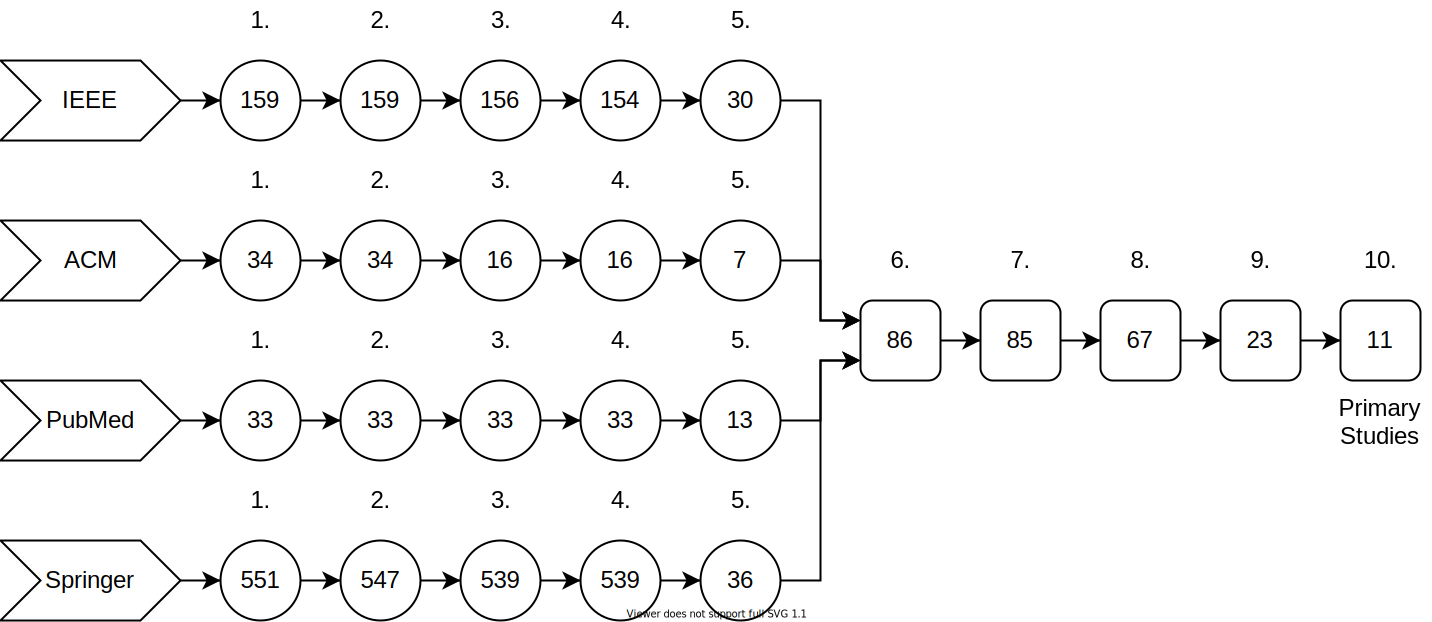
\includegraphics[width=\textwidth]{Imagenes/RR_Steps.svg}
    \includesvg[inkscapelatex=false, width=\textwidth]{Imagenes/RR_Steps.svg}
    \caption{Articles search and selection process details.}
    \label{figura:en/data_extraction}
\end{figure*}

Of a total of 777 articles found, 11 primary studies were analyzed.

\commentcode{The list of the studies analyzed is presented in Table \ref{tabla:en/estudios_primarios}.
\begin{table*}
\setlength\tabcolsep{0pt}
\caption{List of the primary studies analyzed}
\begin{center}
%\resizebox{\columnwidth}{!}{
%\begin{tabular}{|m{2.5em}|m{20em}|}
\begin{tabularx}{\textwidth}{|c|L|}
\hline
\textbf{Id} & \textbf{Primary study} \\
\hline
{[PS1]} & {A. Shaban-Nejad, M. Michalowski, J. S. Brownstein, and D. L. Buckeridge, “Guest editorial explainable ai: Towards fairness, accountability, transparency and trust in healthcare,” IEEE Journal of Biomedical and Health Informatics, vol. 25, no. 7, pp. 2374–2375, Jul. 2021, ISSN: 2168-2208. DOI: 10.1109/JBHI.2021.3088832.} \\
\hline
{[PS2]} & {J. O. O. Ayorinde, F. Citterio, M. Landrò, E. Peruzzo, T. Islam, S. Tilley, G. Taylor, V. Bardsley, P. Li`o, A.Samoshkin, and G. J. Pettigrew, “Artificial intelligence you can trust: What matters beyond performance when applying artificial intelligence to renal histopathology?” eng, Journal of the American Society of Nephrology: JASN, vol. 33, pp. 2133–2140, 12 Dec. 2022. DOI:10.1681/ASN.2022010069.} \\
\hline
{[PS3]} & {A. B. Tosun, F. Pullara, M. J. Becich, D. L. Taylor, J. L. Fine, and S. C. Chennubhotla, “Explainable ai (xai) for anatomic pathology.,” eng, Advances in anatomic pathology, vol. 27, pp. 241–250, 4 Jul. 2020. DOI: 10.1097/PAP.0000000000000264.} \\
\hline
{[PS4]} & {M. H. Jarrahi, V. Davoudi, and M. Haeri, “The key to an effective ai-powered digital pathology: Establishing a symbiotic workflow between pathologists and machine.,” eng, Journal of pathology informatics, vol. 13, p. 100 156, 2022. DOI: 10.1016/j.jpi.2022.100156.} \\
\hline
{[PS5]} & {H. Verma, J. Mlynar, R. Schaer, J. Reichenbach, M. Jreige, J. Prior, F. Evéquoz, and A. Depeursinge, “Rethinking the role of ai with physicians in oncology: Revealing perspectives from clinical and research workflows,” in Proceedings of the 2023 CHI Conference on Human Factors in Computing Systems, ser. CHI'23, Hamburg, Germany: Association for Computing Machinery, 2023, ISBN: 9781450394215. DOI: 10.1145/3544548.3581506. [Online].} \\
\hline
{[PS6]} & {K. A. Tran, O. Kondrashova, A. Bradley, E. D. Williams, J. V. Pearson, and N. Waddell, “Deep learning in cancer diagnosis, prognosis and treatment selection,” en, Genome Medicine, vol. 13, no. 1, p. 152, Dec. 2021, ISSN: 1756-994X. DOI:10.1186/s13073-021-00968-x. [Online].} \\
\hline
{[PS7]} & {W. L. C. dos-Santos, L. A. R. De Freitas, A. A. Duarte, M. F. Angelo, and L. R. Oliveira, “Computational pathology, new horizons and challenges for anatomical pathology,” en, Surgical and Experimental Pathology, vol. 5, no. 1, p. 10, Dec. 2022, ISSN: 2520-8454. DOI:10.1186/s42047-022-00113-x. [Online].} \\
\hline
{[PS8]} & {M. Mohammadi, J. Cooper, O. Arandelovic, C. Fell, D. Morrison, S. Syed, P. Konanahalli, S. Bell, G. Bryson, D. J. Harrison, and D. Harris-Birtill, “Weakly supervised learning and interpretability for endometrial whole slide image diagnosis.,” eng, Experimental biology and medicine (Maywood, N.J.), vol. 247, pp. 2025–2037, 22 Nov. 2022. DOI: 10.1177/15353702221126560} \\
\hline
{[PS9]} & {A. Holzinger, G. Langs, H. Denk, K. Zatloukal, and H. Müller, “Causability and explainability of artificial intelligence in medicine.,” eng, Wiley interdisciplinary reviews. Data mining and knowledge discovery, vol. 9, e1312, 4 Jul. 2019. DOI: 10.1002/widm.1312.} \\
\hline
{[PS10]} & {W. Rösler, M. Altenbuchinger, B. Baeßler, T. Beissbarth, G. Beutel, R. Bock, N. Von Bubnoff, J.N. Eckardt, S. Foersch, C. M. L. Loeffler, J. M. Middeke, M.L. Mueller, T. Oellerich, B. Risse, A. Scherag, C. Schliemann, M. Scholz, R. Spang, C. Thielscher, I. Tsoukakis, and J. N. Kather, “An overview and a roadmap for artificial intelligence in hematology and oncology,” en, Journal of Cancer Research and Clinical Oncology, vol. 149, no. 10, pp. 7997–8006, Aug. 2023, ISSN: 0171-5216, 1432-1335. DOI:10.1007/s00432-023-04667-5. [Online].} \\
\hline
{[PS11]} & {T. Zehra, A. Parwani, J. Abdul-Ghafar, and Z. Ahmad, “A suggested way forward for adoption of AI-Enabled digital pathology in low resource organizations in the developing world,” en, Diagnostic Pathology, vol. 18, no. 1, p. 68, May 2023, ISSN: 1746-1596. DOI:10.1186/s13000-023-01352-6. [Online].} \\
\hline
\end{tabularx}
\label{tabla:en/estudios_primarios}
\end{center}
\end{table*}
}
